\documentclass[a4paper,8pt]{article}

% Packages for formatting
\usepackage{geometry}
\usepackage{float}
\usepackage{array}
\usepackage{lipsum}
% \usepackage{cite}
\geometry{margin=0.5in}
% \usepackage{booktabs}
% \usepackage{bookmark}
\usepackage[table]{xcolor}
\usepackage{graphicx}
% \usepackage{tabularx}
\usepackage{longtable}
\usepackage{amsmath}
\usepackage{caption}

\newcommand\IEEEhyperrefsetup{
bookmarks=true,bookmarksnumbered=true,%
colorlinks=true,linkcolor={black},citecolor={black},urlcolor={blue}%
}
% Preferred hyperref setup, Michael Shell
\usepackage[\IEEEhyperrefsetup, pdftex]{hyperref}
\hypersetup{pdfborder=0 0 0}
% \usepackage{tocloft}

\title{Bill of Materials (BOM) Explanation}
\author{ Pontus Svensson / RoboCup }
\date{\today}

\begin{document}

\maketitle

\newpage
\tableofcontents

\newpage

\section{Introduction}

This document provides an explanation of the Bill of Materials (BOM)
used in the project. Each component listed in the BOM is
described in detail, including its purpose and other relevant
specifications.

\section{BOM}

Table~\ref{table:bom} below outlines the components used in this project along
with their purpose and additional information.
\begin{center}
	\begin{longtable}{|p{3cm}|p{3cm}|p{3cm}|p{1cm}|p{3cm}|p{3cm}|}
		\caption{Main components}
    \label{table:bom}
		\\ \hline \rowcolor{gray!50} \textbf{Component} & \textbf{Description} & \textbf{Purpose} & \textbf{\#} & \textbf{á price (price per robot) SEK} & \textbf{Price in USD}\\ \endhead \hline

		% \rowcolor{gray!50} \textbf{Total price for 1 robot} & \textbf{10457.69} \endlastfoot \hline

		\href{https://www.nanotec.com/fileadmin/files/Datenblaetter/BLDC/DF45/DF45L024048-A.pdf?1656012533}{DF45L024048-A}              & Brushless direct current (BLDC) motor with integrated hall sensors for the wheels & Used to spin the wheels of the robot.                                                                                      & 4  & 830.4 (3273.60) & 74.74 (294.6) \\ \hline
		\href{https://www.hobbywing.com/en/products/xrotor3110}{Hobbywing FPV XRotor 3110 900KV}                                        & Brushless DC motor                                                                & High revolutions per minute (RPM) motor used to control the dribbler.                                                      & 1  & 175.20 (175.20) & 15.77 (15.77) \\ \hline
		\href{https://www.mouser.se/datasheet/2/389/b-g431b-esc1-1848063.pdf}{B-G431B-ESC1}                                             & BLDC motor driver                                                                 & Motor driver with embedded $\mu\text{Controller}$ current sensing and hall sensing to form a closed-loop control algorithm & 5  & 208.96 (1044.8) & 18.8 (94.032) \\ \hline
		\href{https://www.st.com/en/evaluation-tools/nucleo-h723zg.html}{NUCLEO-H723ZG}                                                 & $\mu\text{Controller}$                                                            & Computational power and real-time processing capabilities, supports $\mu\text{ROS}$                                        & 1  & 322.58 (322.58) & 29 (29)       \\ \hline
		\href{https://datasheets.raspberrypi.com/rpi4/raspberry-pi-4-datasheet.pdf}{Raspberry Pi 4 Model B/8GB}                         & Single-board computer                                                             & Processing camera input and performing local path planning                                                                 & 1  & 979 (979)       & 88.11 (88.11) \\ \hline
		\href{https://learn.adafruit.com/adafruit-vl53l4cd-time-of-flight-distance-sensor?view=all}{VL53L4CD ToF}                       & Lidar                                                                             & Obstacle detection (Could not find VL53X ToF)                                                                              & 2  & 176.32 (176.32) & 15.87 (15.87) \\ \hline
		\href{https://www.electrokit.com/upload/product/41013/41013634/DM00112632.pdf}{VL6180 TOF}                                      & Lidar                                                                             & Obstacle detection                                                                                                         & 1  & 39.62 (39.62)   & 3.57 (3.57)   \\ \hline
		\href{https://docs.broadcom.com/doc/AV02-4191EN}{APDS-9960}                                                                     & RGB Sensor                                                                        & Ball detection                                                                                                             & 1  & 199 (199)       & 17.91 (17.91) \\ \hline
		\href{https://wiki.dfrobot.com/BNO055_Intelligent_9_Axis_Sensor_Module_SKU_SEN0374}{SENS0374}                                   & 9-Dof IMU                                                                         & Acceleration, Gyroscope, Magnetometer                                                                                      & 1  & 191 (191)       & 17.19 (17.19) \\ \hline
		\href{https://www.elefun.se/p/prod.aspx?v=65193}{6s 1300mAh -120C - GNB HV XT60}                                                & LiPo-battery                                                                      & Used to power the robot                                                                                                    & 1  & 351.20 (351.20) & 31.6 (31.6)   \\ \hline
		\href{https://www.ichaus.de/product/ic-px-series/#documents}{iC-PX2604 + PX01S 26-30}                                           & Wheel encoders                                                                    & Will be used for odometry and determining the RPM                                                                          & 4  & 224.40 (897.60) & 20.2 (80.78)  \\ \hline
		\href{https://www.we-online.com/components/products/datasheet/2536030320001.pdf}{WSEN-ISDS 6 Axis IMU}                          & 6-DoF IMU                                                                         & Will be used for odometry of the robot                                                                                     & 10 & N/A             & N/A           \\ \hline
		\href{https://www.electrokit.com/upload/product/41020/41020240/Camera_Module_3_Product_Brief.pdf}{Raspberry Pi Camera-module 3} & Camera                                                                            & Provide images in front of the robot to detect the ball and obstacles                                                      & 1  & 369 (369)       & 33.21 (33.21) \\ \hline
	\end{longtable}
\end{center}
\section{Reason for component choice}

\subsection{DF45L024048-A}

% SSL robot motor characteristic
During competition a SSL-robot is most of the time accelerating
\cite{francaRob^oCInSmallSize}. Having a motor which can provide
sufficient torque at any given speed is crucial.

% DF45L024048-A introduction
The DF45L024048-A BLDC motors provides a good tradeoff between torque
and RPM, with integrated hall sensors. The sensors detect the position
of the rotor relative to the stator which gives the ability to control
the motors using commutation. The motor controller uses the signals
from the hall sensors to determine the exact timing for switching the
current in the stator windings. This gives a smooth motor operation
while maximizing torque output.

% Other considerations
The size of the motor has to be taken into account. Having to
large footprint on the motors would cause the kicker (solenoid) to not
fit in the chassi. Using a general 5010 sensorless drone motor could
be used as demonstrated by \cite{veeraghanta2024TeamDescription} but
this motor would require a more sophisticated ESC which would take a
lot of time to develop and manufacture. The problem with searching for
5010 drone motors is that most websites does not show the
full torque graph, they primarly show the torque when the motor is
already spinning at $40\%$ throttle and above. Therefore finding a 5010 drone
motor with adequate torque at low speeds is deceptively difficult.

% Provide sources for my claims
Using hall sensors is a common method utilized by several teams and
proven to be a winning concept \cite{ryllExtendedTeamDescription}\cite{abiyevNEUIslandersTeamDescription}\cite{wuCompilationErrorTeam}\cite{francaRob^oCInSmallSize}.

% Dribbler
\subsection{Hobbywing FPV XRotor 3110 900KV}

% Dribbler requirements
The requirements for the dribbler motor is that it can reach high RPM
(around $10\:000\text{ RPM}$). No feedback is implemented for the
dribbler motor, due to the timeframe of the project a control algorithm will not be implemented.

% Motor driver
\subsection{B-G431B-ESC1}

% Sensorless controller hiccups
A sensorless controller requires that the BLDC motor produce a
measurable back electromotive force (EMF) so the controller can
determine the position of the rotor and therefore cannot provide
smooth commutation at start up and low speeds.
\cite{roweInstrumentationControlHigh2012}

% Introduction to B-G431B-ESC1
The chosen electronics speed controller (ESC) has an STSPIN32F0A
system in package chip which has an integrated STM32 processor with
hall sensor decoding logic and current sensing capabilities. This
makes this ESC a good fit with the DF45L024048-A BLDC motor.

% STSPIN32F0A
The STSPIN32F0A chip is a common choice for controlling BLDC motors in
the SSL competitions which has been proven to be reliable and
succesful
\cite{ryllExtendedTeamDescription}\cite{abousaleh2024TeamDescription}.

% FOC
Field-Oriented control (FOC) can be implemented on the B-G431B-ESC1. Guidance and firmware for the B-G431B-ESC1 has been received from Delft Mercurians that will make the process of implementing this streamlined.

% PID system
A PID system can be implemented on the chip to allow for precise
movement and rapid acceleration which is critical to make fast
directions changes.

% Implementation plan of the PID
The B-G431B-ESC1 will receive a desired velocity, to use this within
a PID system the RPM of each motor is required.

% Size and weight
The size and weight of the ESC does also have to be taken in
consideration, the B-G431B-ESC1 has a small footprint with a
relatively low weight $286\text{g}$. With all the components
integrated on one board will make the assembly process easier and
reduce any external components e.g. hall sensing or mosfets. The
programming for the integrated STM32 is done using STM32 Motor Control
Software Development Kit which is a graphical programming environtment
from ST.

\subsection{NUCLEO-H723ZG Microcontroller}

The \text{NUCLEO-H723ZG} is a development board based on the
STM32H723ZG chip, it comes with all necessary peripheral communication
UART, SPI, I2C and CAN. The STM32H723ZG features an ARM Cortex-M7 core
operating at up to 480 MHz, providing good processing power for
handling multiple real-time tasks required in our application.

Additionally, the STM32 series is widely adopted in RoboCup
competitions, including the \textbf{Small Size League (SSL)} \cite{ryllExtendedTeamDescription}\cite{zhaoZJUNlictExtendedTeam}\cite{wuCompilationErrorTeam}.
This widespread use underscores its reliability and effectiveness in
competititions. By using STM32H723ZG chip, previous teams implementations that is open sourced can be used for guidance when developing.

To manage the various tasks and ensure smooth operation of our robot,
the control architecture will be implemeted using \textbf{micro-ROS} in
combination with \textbf{FreeRTOS} on the NUCLEO-H723ZG.

\textbf{FreeRTOS} is a real-time operating system that provides task
scheduling and resource management. Implementing FreeRTOS on the
NUCLEO-H723ZG allows us to handle multiple concurrent tasks
efficiently, such as sensor data processing, motor control, and
communication with other system components.

By using the STM32H723ZG chip future improvements can be made, without having to replace the hardware and potentially the need to re-program/port using another framework.

% \subsubsection{UdeA collaboration}
%
% UdeA will be programming on the ESP32-S3 with FreeRTOS as their framework. Their proposed method for motor control is to use a AS5600 sensor for each motor to measure the RPM and using the ESP32-S3 to create a closed-loop control algorithm.
%
% This will be a similar implementation to our intended control-algorithm. We will use an optical wheel encoder to measure the RPM, and will be used as feedback to create a closed-loop PID algorithm.
%
% From our perspective the programming that is required for this is similar to UdeA. And thus we could still collaborate even though the microcontroller is different.
%
% I have also not found any teams that have used the ESP32 as their main processor, and almost every team uses STM32 based controller or a Raspberry Pi compute module.

\subsection{Raspberry Pi 4 Model B/8GB}

It is important to accurately detect the ball and other robots in a
timely manner, therefore a Raspberry Pi camera will be used, and the input image
will be processed on the Raspberry Pi 4. The Raspberry pi has
been used in the SSL competitions for this purpose
\cite{ommerExtendedTeamDescription}\cite{satoGreenTea2024Team}. A lot of information and open sourced firmware exist.

The Raspberry Pi 4 was also chosen to be able to run the DWA path
planning algorithm, due to the timeframe of this project, implementing
DWA by ourself would require too much time.

% \subsubsection{UdeA considerations}
%
% UdeA has chosen two different components, TOF400C-VL53L1 and VL6180 TOF that is going to be used for obstacle detection and ball detection. Since we are going to run computationally intensive tasks on the Raspberry Pi, replacing it would disrupt a lot of our planning between the software and hardware team.
%
% Our proposed idea is that we can add these components for extra input to allow us to collaborate when developing the software for these components. 

\subsection{VL53L4CD ToF Sensor}

The \textbf{VL53L4CD ToF} (Time-of-Flight) sensor is a laser-based ranging sensor capable of measuring distances with high accuracy. It is used for obstacle detection in the robot, allowing the system to identify obstacles within close proximity. With a range of up to 1300 mm, it is especially suited for detecting obstacles that could interfere with the robot's navigation. The sensor communicates using I2C, which simplifies integration with the existing hardware.

\subsection{VL6180 TOF Sensor}

The \textbf{VL6180 TOF} sensor, also a Time-of-Flight sensor, serves a similar purpose as the VL53L4CD but operates at shorter distances, making it ideal for near-field obstacle detection. It is also chosen for its compact size and I2C communication, which allows it to seamlessly interface with the microcontroller. The shorter range provides additional resolution for objects very close to the robot, further enhancing obstacle detection accuracy.

\subsection{APDS-9960 Sensor}

The \textbf{APDS-9960} sensor is a versatile RGB sensor with integrated IR sensing capabilities. It is primarily used in this project for ball detection, as it can distinguish colors and detect the presence of nearby objects. This feature enables the robot to differentiate the ball from the surroundings based on color and proximity. Communication is handled via I2C, allowing for easy connection to the system’s microcontroller.

\subsection{SENS0374 Sensor}

  The \textbf{SENS0374}, based on the Bosch BNO055 sensor, is a 9-axis absolute orientation sensor module. It integrates a triaxial accelerometer, gyroscope, and geomagnetic sensor with a 32-bit microcontroller, providing orientation data essential for stable navigation and localization. The module includes an onboard fusion algorithm that combines sensor readings to deliver absolute orientation, minimizing drift over time. The SENS0374 communicates via I2C and SPI, making it flexible for integration with the main controller. This sensor will aid in tracking the robots movement, orientation, and any external forces acting upon it, enhancing its responsiveness in dynamic environments.

\subsection{SX1280IMLTRT + SKY66122-11}

To obtain a reliable connection to the team server, the SX1280IMLTRT RF transceiver with the SKY66122-11
front-end-module is used.

This implementation has been proven succesful by several teams \cite{ryllExtendedTeamDescription}\cite{barretoRoboIMEIgnitingInnovation}.

However, to implement this, a basestation is required and due to the time limitation of this project it is not feasible to design and write firmware for our own network protocol, but these components will be added to the mainboard PCB for future iterations. The communication will instead be done using the wifi on the Raspberry Pi 4.

% \subsubsection{UdeA considerations}
%
% I have not yet gotten it confirmed how UdeA has planned to communicate with the server laptop. But from my assumption they will use the WiFi card placed on the ESP32-S3. 
%
% Teams have acknowledged the difficulties with enabling a reliable connection to the team server, when using components like the nRF52 and Raspberry Pis. Teams that did use the ESP32 for WiFi communication also faced a lot of problems \cite{bhatKgpKubs2020Team}.
%
% Therefore we have opted for a different route that has been used by several teams and proven to be reliable\cite{ryllExtendedTeamDescription}.
%
\subsection{iC-PX2604 + PX01S 26-30}

This wheel encoder comes as a complete module which will be easy to
integrate and in combination with the NUCLEO-H723ZG the resolution of
the encoder is increased.

Optical wheel encoders is commonly used by teams competing in the SSL competitions.

% \subsubsection{UdeA considerations}
%
% UdeA has chosen to use the AS5600 magnetic encoder. This setup requires that a magnet is glued to the end of the shaft for every motor. This process also require that the magnet aligns properly and does not come loose during movement and vibrations. We have not gotten more information about how they intended to attach this sensor.
%
% Therefore we would opt for using our optical wheel encoders instead since the integration is done with the wheel assembly and will attach using screws, making the assembly streamlined. Both sensor will be able to provide sensor values that can be used for RPM estimations and odometry.
%
\subsection{WSEN-ISDS 6 Axis IMU}

The IMU chosen is supplied free of charge from Würth
electronics. It communicates using I2C or SPI which both are available
on the NUCLEO-H723ZG.

% \subsubsection{UdeA considerations}
%
% UdeA has chosen to use two different 9-Dof IMUs, however since we got our IMUs free of charge it is smarter to just use those. They did not mention anything about these sensor during our BOM meeting.
% The implementation of the sensors will be similar to some degree both our IMU and BNO055 IMU supports I2C as communication protocol.

\subsection{Raspberry Pi Camera-module 3}

The Raspberry Pi camera-module 3 is chosen because of its seamless
integration with the Raspberry Pi 4.

% \subsection{IR Break Beam Sensor - 5mm LEDs}
%
% The IR Break Beam sensor will be connected using GPIO pins on the
% NUCLEO-H723ZG with a pull-up resistor. To detect if the ball is touching the dribbler roller.

% \subsubsection{UdeA considerations}
%
% UdeA has chosen to use GY-9960-3.3 APDS-9960 RGB sensor. They did not specify how this is going to be used or implemented during our meeting about their BOM.
%
% We have decided not to include this sensor in our desired BOM since it is unclear what the purpose is.

% \subsection{Connectors}
%
% Connectors for the main PCB board will be supplied by Würth
% electronics.
%
% \subsection{Shaft hub with clamping bracket 4mm}
%
% From our research teams have noticed that if the coupling between the
% motorshaft and wheels does not have a good fit, the shaft will start
% to release tiny metal dust which will be collected by the hub of the
% BLDC motor.
%
% Therefore we have chosen to use this clamp to ensure the coupling is
% secure.
%
% \subsection{Bearings}
%
% Bearings used for the roller.
%
% \subsection{Resistors}
%
% Any Passive components required will be supplied by Würth electroncis
% or if we can find it in 326.
%
% \subsection{Capacitors}
%
% Any Passive components required will be supplied by Würth electroncis
% or if we can find it in 326.
%
% \subsection{Voltage regulators}
%
% The voltage regulators will be used to ensure our components reveice
% the correct voltages, 3.3V, 5V, 12V will be integrated on the custom
% PCB.
%
% The voltage regulators was supplied by Würth electronics.
%
% \subsection{Solenoid}
%
A custom made solenoid would be preferred, but due to time a
generic solenoid will be used for starting car engines.
Supplied by MDU.

\subsection{PCB}

As some of our components require a custom PCB, three PCBs will be designed. A mainboard, kicker-board and encoder board, the main board will host
connectors for the battery, motors, sensors, NUCLEO-H723ZG and pin headers for
powering the Raspberry Pi. The mainboard will also host the RF
transceiver, IMU and voltage regulators.

\section{Hardware Architecture}

Figure~\ref{fig:hardware_architecture} depicting the hardware
architecture of the proposed robot.

\begin{figure}[H]
	\begin{center}
		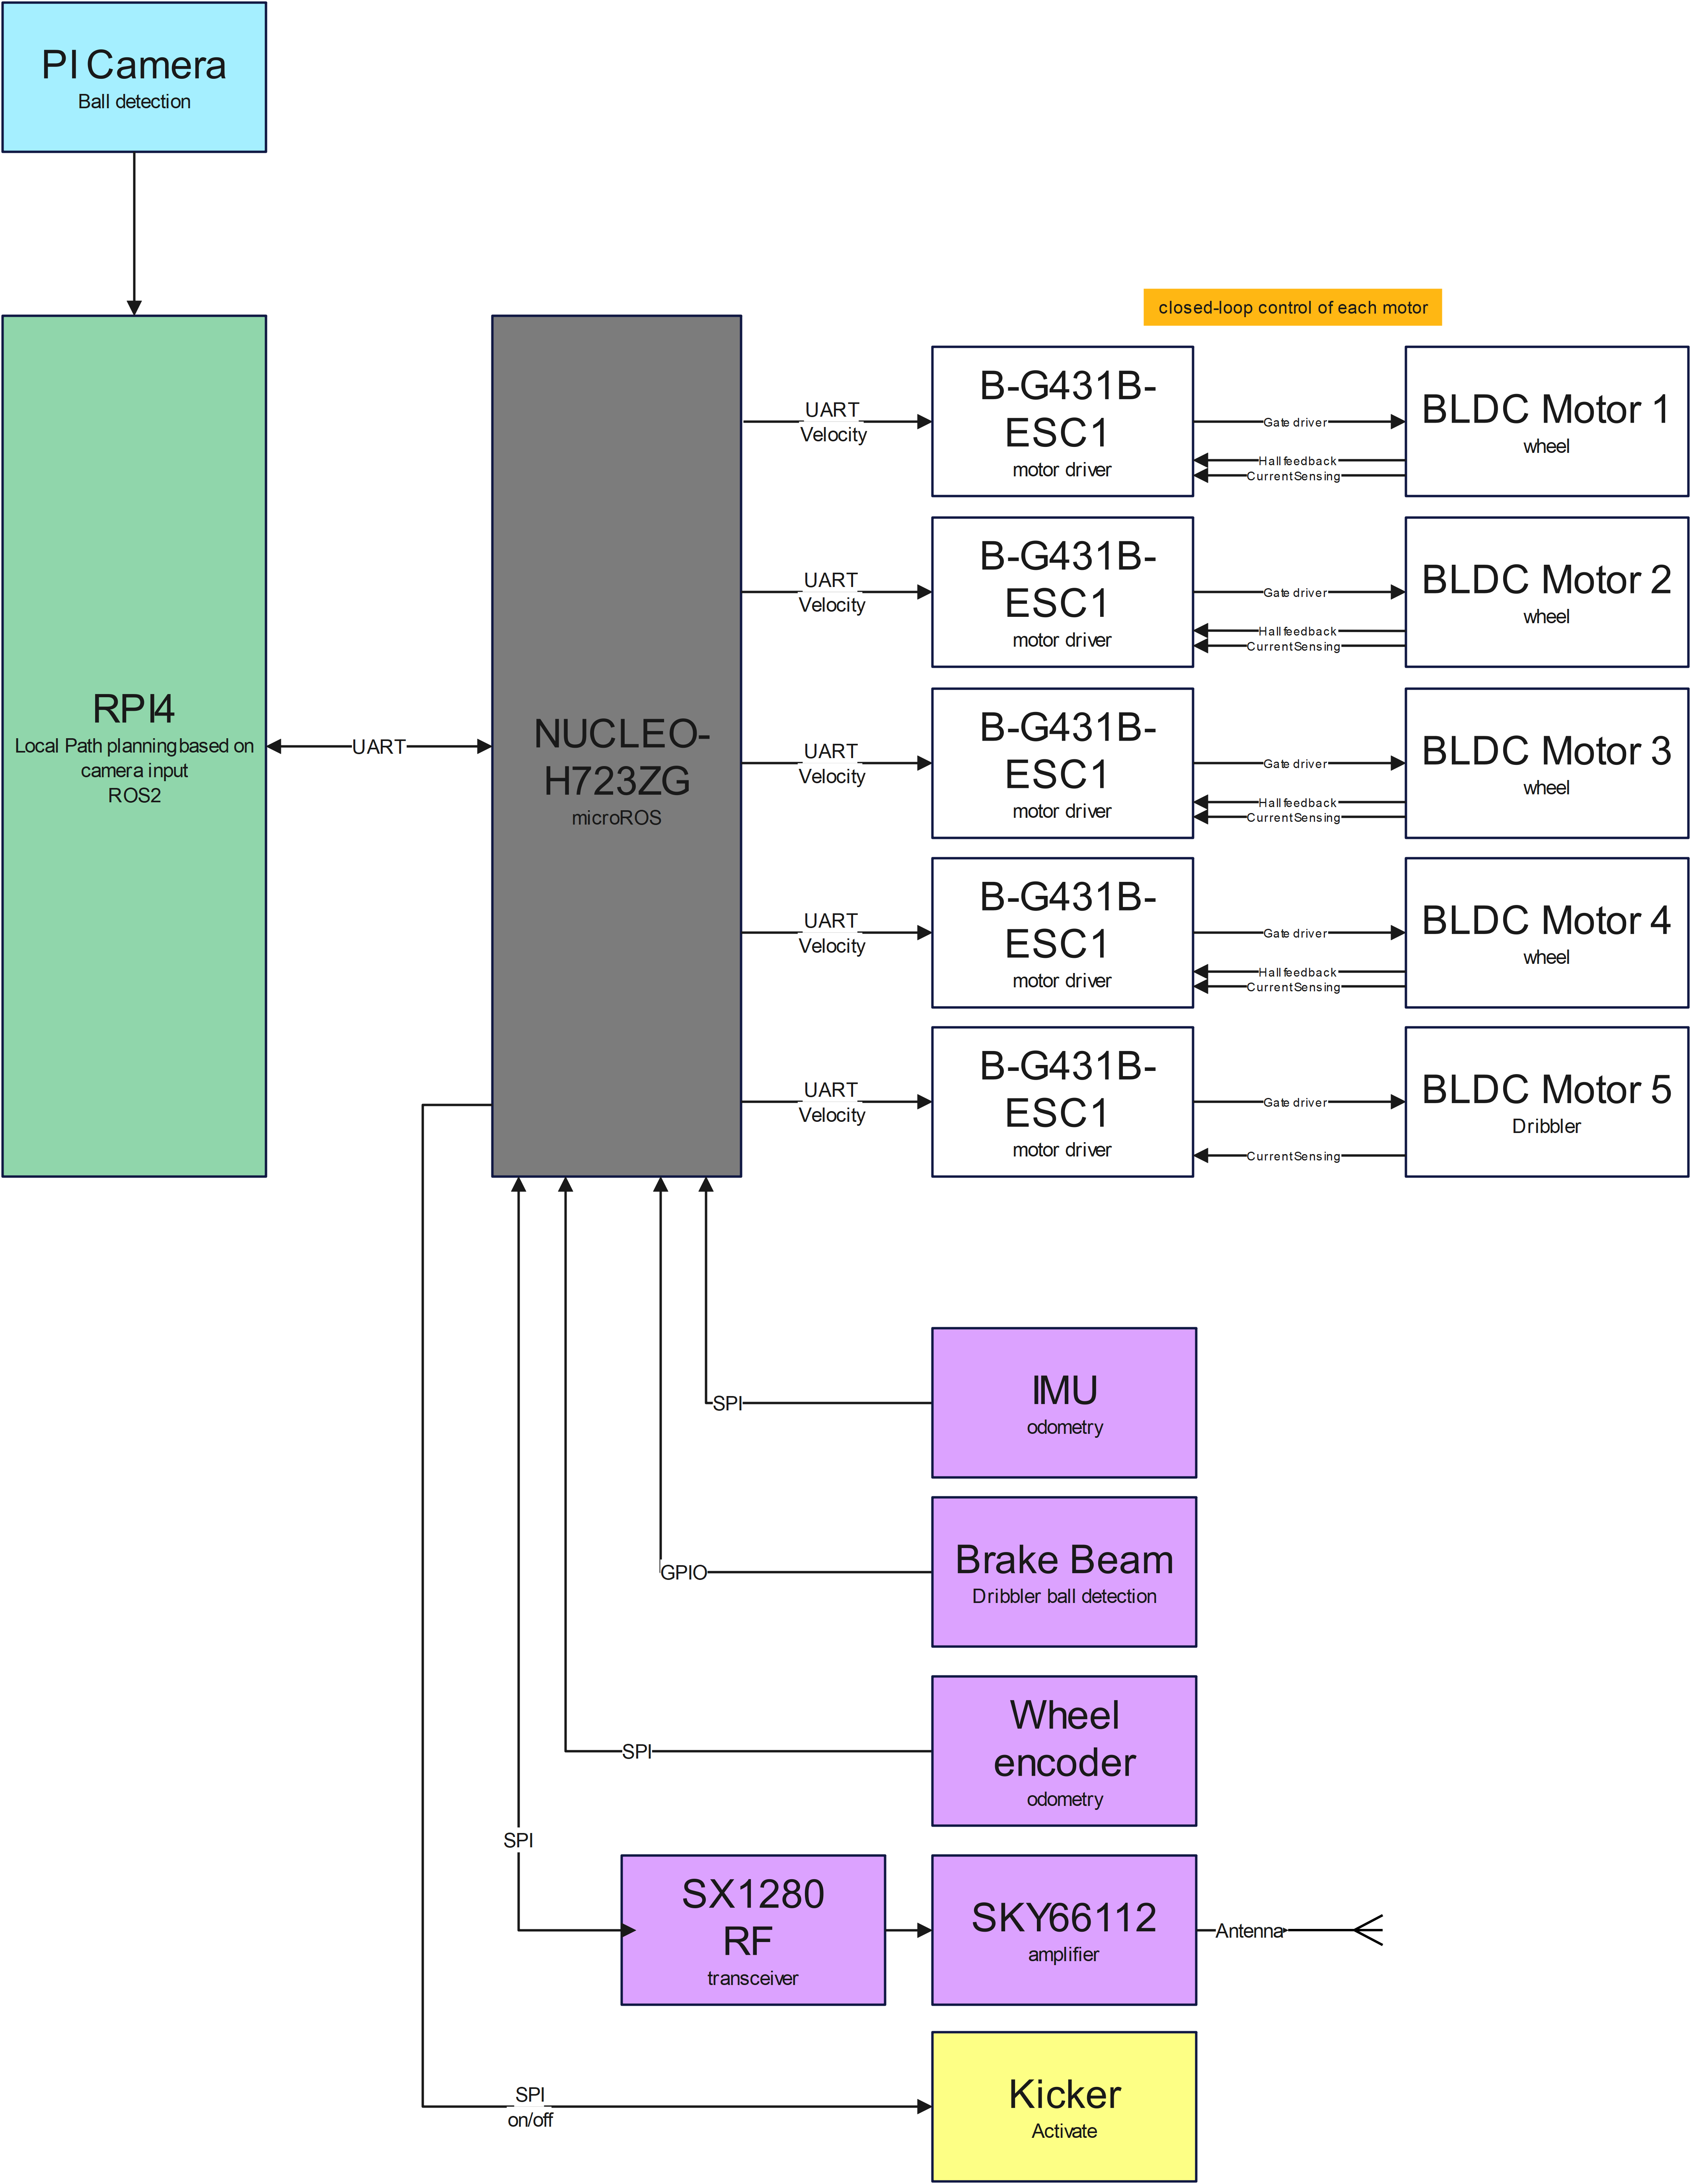
\includegraphics[width=0.5\textwidth]{Hardware_architecture.png}
	\end{center}
	\caption{Hardware Architecture}
	\label{fig:hardware_architecture}
\end{figure}

\bibliographystyle{IEEEtran} \bibliography{DVA490_DVA474}
\end{document}
